\documentclass[a3paper,12pt]{extarticle} % Use extarticle for A3 paper size
\usepackage{graphicx} % Include this package for \includegraphics
\usepackage{amsmath}
\usepackage{amssymb} % Include this package for \mathbb
\usepackage[margin=1in]{geometry} % Adjust the margin as needed

\begin{document}

\author{kipngeno koech - bkoech}
\title{Homework 0 - Introduction to Probabilistic Graphical Models}   
\maketitle

\medskip

\maketitle

\section{Probability}
\begin{enumerate}
    \item A fair coin is tossed 10 times. The sample space for each trial is Head, Tail and the trials are independent. What is the probability of having:
    \[
        P(H) = \frac{1}{2}, \quad P(T) = \frac{1}{2}
    \]
    The probability of getting exactly \( k \) heads
    is given by the binomial distribution:
    \[
        P(X = k) = \binom{n}{k} p^k (1-p)^{n-k}
    \]
    where \( n = 10 \) and \( p = \frac{1}{2} \).
    \begin{enumerate}
        \item Zero Tail
        \[
            P(0T) = \binom{10}{0} \left(\frac{1}{2}\right)^0 \left(\frac{1}{2}\right)^{10} = \frac{1}{1024}
        \]
        \item 6 heads
        \[
            P(6H) = \binom{10}{6} \left(\frac{1}{2}\right)^6 \left(\frac{1}{2}\right)^4 = \frac{210}{1024}
        \]
        \item At least three heads
        \[
            P(X \geq 3) = 1 - P(X < 3) = 1 - P(X = 0) - P(X = 1) - P(X = 2) = 1 - \left(\frac{1}{1024} + \frac{10}{1024} + \frac{45}{1024}\right) = \frac{968}{1024}
        \]
        \item At least three Heads given the first trail was a Head!
        \[
            P(X \geq 3 | X_1 = H) = 1 - P(X < 3 | X_1 = H) = 1 - P(X = 0 | X_1 = H) - P(X = 1 | X_1 = H) - P(X = 2 | X_1 = H) = 1 - \left(\frac{1}{512} + \frac{9}{512} + \frac{36}{512}\right) = \frac{466}{512}
        \]
        \[
         = 1 - \left(\frac{1}{512} + \frac{9}{512} + \frac{36}{512}\right) = \frac{466}{512}
        \]
    \end{enumerate}
    \item Assuming the probability that it rains on Monday is 0.45; the probability that it rains on Wednesday is 0.4; and the probability that it rains on Wednesday given that rained on Monday is 0.6. What is the probability that:
    \begin{enumerate}
        \item It rains on both days
        \[
            P(M \cap W) = P(W | M)P(M) = 0.6 \times 0.45 = 0.27
        \]
        \item Rain will come next Monday, given that it has just finished raining today (Wednesday)
        \[
            P(M | W) = \frac{P(W | M)P(M)}{P(W)} = \frac{0.6 \times 0.45}{0.4} = 0.675
        \]
    \end{enumerate}
    \item Let \(X\) denote the outcome of a random experiment with possible values \{-4, -3, -2, -1, 0, 1, 2, 3, 4\} according to the following probability law:
    \[
        P(X = k) = 
    \begin{cases}
        ck^2 & \text{if } k \in \{-4, -3, -2, -1, 0, 1, 2, 3, 4\} \\
        0 & \text{otherwise}
    \end{cases}
    \]
    \begin{enumerate}
        \item What is the value of \(c\)?
        \[
            \sum_{x \in \{-4, -3, -2, -1, 0, 1, 2, 3, 4\}} P(X = k) = 1
        \]
        Total proabability is 1:
        \[
            \sum_{k \in \{-4, -3, -2, -1, 0, 1, 2, 3, 4\}} ck^2 = 1
        \]
        \[
            c \sum_{k \in \{-4, -3, -2, -1, 0, 1, 2, 3, 4\}} k^2 = 1
        \]
        \[
            c \times( (-4)^2 + (-3)^2 + (-2)^2 + (-1)^2 + 0^2 + 1^2 + 2^2 + 3^2 + 4^2) = 1
        \]
        \[
            c \times( 16 + 9 + 4 + 1 + 0 + 1 + 4 + 9 + 16) = 1
        \]
        \[
            c \times 60 = 1
        \]
        \[
            c = \frac{1}{60}
        \]
        
        \item Compute the expectation and variance of \(X\).
        \\\textbf{Expectation:}
        \[
            E[X] = \sum_{k \in \{-4, -3, -2, -1, 0, 1, 2, 3, 4\}} kP(X = k)
        \]
        \[
            E[X] = \sum_{k \in \{-4, -3, -2, -1, 0, 1, 2, 3, 4\}} k \times \frac{k^2}{60}
        \]
        \[
            E[X] = \frac{1}{60} \sum_{k \in \{-4, -3, -2, -1, 0, 1, 2, 3, 4\}} k^3
        \]
        \[
            E[X] = \frac{1}{60} \times (-4^3 - 3^3 - 2^3 - 1^3 + 0^3 + 1^3 + 2^3 + 3^3 + 4^3)
        \]
        \[
            E[X] = \frac{1}{60} \times (-64 - 27 - 8 - 1 + 0 + 1 + 8 + 27 + 64)
        \]
        \[
            E[X] = \frac{1}{60} \times 0 = \textbf{0}
        \]
        \\\textbf{Variance:}
        \[
            Var(X) = E[X^2] - E[X]^2
        \]
        \[
            E[X^2] = \sum_{k \in \{-4, -3, -2, -1, 0, 1, 2, 3, 4\}} k^2P(X = k)
        \]
        \[
            E[X^2] = \sum_{k \in \{-4, -3, -2, -1, 0, 1, 2, 3, 4\}} k^2 \times \frac{k^2}{60}
        \]
        \[
            E[X^2] = \frac{1}{60} \sum_{k \in \{-4, -3, -2, -1, 0, 1, 2, 3, 4\}} k^4
        \]
        \[
            E[X^2] = \frac{1}{60} \times (-4^4 - 3^4 - 2^4 - 1^4 + 0^4 + 1^4 + 2^4 + 3^4 + 4^4)
        \]
        \[
            E[X^2] = \frac{1}{60} \times (256 + 81 + 16 + 1 + 0 + 1 + 16 + 81 + 256)
        \]
        \[
            E[X^2] = \frac{1}{60} \times 708 = 11.8
        \]
        \[
            Var(X) = E[X^2] - E[X]^2 = 11.8 - 0 = \textbf{11.8}
        \]

        
    \end{enumerate}
    \item ou just built a new COVID test with the following properties:
    \begin{itemize}
        \item If a person has COVID, the test is positive with  0.95 probability.
        \item If a person does not have COVID, the test can still be positive with 0.05 probability.
    \end{itemize}
    You are told that a random person has COVID with probability 0.001. You just use your test on a random person and it turns out to be positive. What is the probability that the person really has COVID?
    \[
        P(C) = 0.001, \quad P(\bar{C}) = 0.999
    \]
    \[
        P(T | C) = 0.95, \quad P(T | \bar{C}) = 0.05
    \]
    Bayes theorem:
    \[
        P(C | T) = \frac{P(T | C)P(C)}{P(T)}
    \]
    Probability of a positive test( Total Probability):
    \[
        P(T) = P(T | C)P(C) + P(T | \bar{C})P(\bar{C}) = 0.95 \times 0.001 + 0.05 \times 0.999 = 0.0509
    \]
    so:
    \[
        P(C | T) = \frac{0.95 \times 0.001}{0.0509} = \textbf{0.0186}
    \]
    \item You will write a python program to simulate the Monthy Hall problem. It’s a famous problem, and you can read more about it online. Suppose you’re on a game show, and you’re given the choice of three doors: Behind one door is a car; behind the others, goats. You pick a door (but don’t open it)s, say No. 1, and the host, who knows what’s behind the doors, opens another door, say No. 3, which has a goat. He then says to you, ”Do
    you want to pick door No. 2?” Is it to your advantage to switch your choice? In this simulation, the doors will be represented by an array of three elements. Each element of the
    array is either a ”0” (for the goats) or a ”1” (for the car). A python file is provided with four functions to fill.
\end{enumerate}

\newpage
\section{MLE-MAP (Warmup)}

Suppose that \( x \in \mathbb{R}^d \) is fixed and given. Moreover, assume that \( \beta \in \mathbb{R}^d \) is a parameter vector and
\[
y = \langle x, \beta \rangle + \epsilon, \quad \text{where} \quad \epsilon \sim \mathcal{N}(0, \sigma^2),
\]
where \( \langle \cdot, \cdot \rangle \) denotes the inner (i.e., dot) product of two vectors, that is, if \( \beta = \begin{pmatrix} \beta_1 & \beta_2 & \cdots & \beta_d \end{pmatrix}^T \) and
\( x = \begin{pmatrix} x_1 & x_2 & \cdots & x_d \end{pmatrix}^T \), then \( \langle x, \beta \rangle = \sum_{i=1}^d x_i \beta_i \).
Therefore, \( y \) is a linear function of \( x \) with i.i.d. Gaussian noise.

\begin{enumerate}
    \item \textbf{Maximum likelihood estimation:}
    \begin{enumerate}
        \item Write down the probability density function (PDF) of the conditional distribution \( y | \beta \). Your answer can be in terms of the fixed \( x \in \mathbb{R}^d \).
        \[
            f(y | \beta) = \frac{1}{\sqrt{2 \pi \sigma^2}} \exp \left( -\frac{(y - \langle x, \beta \rangle)^2}{2 \sigma^2} \right)
        \]

        \item Assume that we (independently) draw \( N \) pairs \( (x_n, y_n) \in \mathbb{R}^d \times \mathbb{R} \) from the above model, where \( x_n \)'s are fixed and then \( y_n \) is defined according to:
        \[
            y_n = \langle x_n, \beta \rangle + \epsilon_n, \quad \text{where} \quad \epsilon_n \sim \mathcal{N}(0, \sigma^2)
        \]
        What is the PDF of \( (y_1, \ldots, y_N | \beta) \)?
        \[
            f(y_1, \ldots, y_N | \beta) = \prod_{n=1}^N \frac{1}{\sqrt{2 \pi \sigma^2}} \exp \left( -\frac{(y_n - \langle x_n, \beta \rangle)^2}{2 \sigma^2} \right)
        \]

        \item Write down the associated log-likelihood function for the PDF you found in part (b).
        \[
            \log \mathcal{L}(\beta) = \log \left( \prod_{n=1}^N \frac{1}{\sqrt{2 \pi \sigma^2}} \exp \left( -\frac{(y_n - \langle x_n, \beta \rangle)^2}{2 \sigma^2} \right) \right)
        \]
        \[
            \log \mathcal{L}(\beta) = \sum_{n=1}^N \left( -\frac{1}{2} \log (2 \pi \sigma^2) - \frac{(y_n - \langle x_n, \beta \rangle)^2}{2 \sigma^2} \right)
        \]
        \[
            \log \mathcal{L}(\beta) = -\frac{N}{2} \log (2 \pi \sigma^2) - \frac{1}{2 \sigma^2} \sum_{n=1}^N (y_n - \langle x_n, \beta \rangle)^2
        \]

        \item Find \( \beta \) that maximizes the log-likelihood function from part (c).
        \[
            \hat{\beta} = \arg \max_{\beta} \log \mathcal{L}(\beta)
        \]
        \[
            \hat{\beta} = \arg \min_{\beta} \sum_{n=1}^N (y_n - \langle x_n, \beta \rangle)^2
        \]
        \[
            \hat{\beta} = (X^T X)^{-1} X^T y
        \]
        where \( X \) is the matrix with rows \( x_n^T \) and \( y \) is the vector with elements \( y_n \).
    \end{enumerate}
    \item \textbf{Maximum a posteriori estimation:}
    \begin{enumerate}
        \item \textbf{Maximum a posteriori estimation:}
        \begin{enumerate}
            \item Assume \( \beta \sim \mathcal{N}(0, \lambda^2 I_d) \) where \( I_d \) is the \( d \times d \) identity matrix.
            After drawing \( N \) pairs as above, from Bayes' rule we know the distribution of \( \beta | (y_1, \ldots, y_N) \) is
            \[
                P(\beta | y_1, \ldots, y_N) = \frac{P(y_1, \ldots, y_N, \beta)}{P(y_1, \ldots, y_N)}
            \]
            Find the distribution \( P(y_1, \ldots, y_N, \beta) \).

            The joint distribution \( P(y_1, \ldots, y_N, \beta) \) can be written as:
            \[
                P(y_1, \ldots, y_N, \beta) = P(y_1, \ldots, y_N | \beta) P(\beta)
            \]
            From the previous part, we have:
            \[
                P(y_1, \ldots, y_N | \beta) = \prod_{n=1}^N \frac{1}{\sqrt{2 \pi \sigma^2}} \exp \left( -\frac{(y_n - \langle x_n, \beta \rangle)^2}{2 \sigma^2} \right)
            \]
            And since \( \beta \sim \mathcal{N}(0, \lambda^2 I_d) \), we have:
            \[
                P(\beta) = \frac{1}{(2 \pi \lambda^2)^{d/2}} \exp \left( -\frac{\|\beta\|^2}{2 \lambda^2} \right)
            \]
            Therefore,
            \[
                P(y_1, \ldots, y_N, \beta) = \left( \prod_{n=1}^N \frac{1}{\sqrt{2 \pi \sigma^2}} \exp \left( -\frac{(y_n - \langle x_n, \beta \rangle)^2}{2 \sigma^2} \right) \right) \left( \frac{1}{(2 \pi \lambda^2)^{d/2}} \exp \left( -\frac{\|\beta\|^2}{2 \lambda^2} \right) \right)
            \]

            \item Note that from Bayes' rule, finding the MAP estimator of \( \beta \) is equivalent to maximizing the numerator \( P(y_1, \ldots, y_N, \beta) \) with respect to \( \beta \) since the denominator does not depend on \( \beta \). Use the expression from part (a) above to formulate a minimization problem whose solution will give the MAP estimator \( \hat{\beta} \).

            To find the MAP estimator \( \hat{\beta} \), we need to maximize \( P(y_1, \ldots, y_N, \beta) \) with respect to \( \beta \). This is equivalent to minimizing the negative log of \( P(y_1, \ldots, y_N, \beta) \):
            \[
                \hat{\beta} = \arg \max_{\beta} P(y_1, \ldots, y_N, \beta)
            \]
            \[
                \hat{\beta} = \arg \min_{\beta} -\log P(y_1, \ldots, y_N, \beta)
            \]
            \[
                -\log P(y_1, \ldots, y_N, \beta) = -\log \left( \prod_{n=1}^N \frac{1}{\sqrt{2 \pi \sigma^2}} \exp \left( -\frac{(y_n - \langle x_n, \beta \rangle)^2}{2 \sigma^2} \right) \right) - \log \left( \frac{1}{(2 \pi \lambda^2)^{d/2}} \exp \left( -\frac{\|\beta\|^2}{2 \lambda^2} \right) \right)
            \]
            \[
                -\log P(y_1, \ldots, y_N, \beta) = \sum_{n=1}^N \left( \frac{(y_n - \langle x_n, \beta \rangle)^2}{2 \sigma^2} + \frac{1}{2} \log (2 \pi \sigma^2) \right) + \frac{\|\beta\|^2}{2 \lambda^2} + \frac{d}{2} \log (2 \pi \lambda^2)
            \]
            Ignoring the constant terms that do not depend on \( \beta \), we get:
            \[
                \hat{\beta} = \arg \min_{\beta} \left( \sum_{n=1}^N \frac{(y_n - \langle x_n, \beta \rangle)^2}{2 \sigma^2} + \frac{\|\beta\|^2}{2 \lambda^2} \right)
            \]
            \[
                \hat{\beta} = \arg \min_{\beta} \left( \frac{1}{2 \sigma^2} \sum_{n=1}^N (y_n - \langle x_n, \beta \rangle)^2 + \frac{1}{2 \lambda^2} \|\beta\|^2 \right)
            \]
            \[
                \hat{\beta} = \arg \min_{\beta} \left( \sum_{n=1}^N (y_n - \langle x_n, \beta \rangle)^2 + \frac{\sigma^2}{\lambda^2} \|\beta\|^2 \right)
            \]
            Therefore, the MAP estimator \( \hat{\beta} \) is the solution to the following minimization problem:
            \[
                \hat{\beta} = \arg \min_{\beta} \left( \sum_{n=1}^N (y_n - \langle x_n, \beta \rangle)^2 + \frac{\sigma^2}{\lambda^2} \|\beta\|^2 \right)
            \]
        \end{enumerate}

    \end{enumerate}
\end{enumerate}

\newpage
\section{Graph Theory}
\begin{enumerate}
    \item Degree of any Vertex of a graph is:
    \[
        \text{ (b) The number of edges incident with the vertex}
    \]
    \item In each of the following Graphs, find paths of lenght 9 and 11, and cycles of length 5, 6, 8 and 9 if possible.
    \begin{figure}[h!]
        \centering
        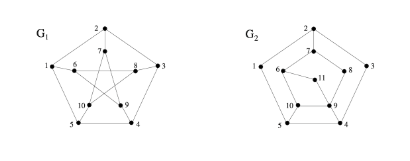
\includegraphics[width=0.8\textwidth]{PGM-graph.png}
        \caption{Graph for finding paths and cycles}
        \label{fig:pgm-graph}
    \end{figure}
    \\
    G1:
    \[
        \text{Paths of length 9: } 1 \rightarrow 2 \rightarrow 3 \rightarrow 8\rightarrow 6 \rightarrow 9 \rightarrow 4 \rightarrow 5 \rightarrow 10
    \]
    \[
        \text{Paths of length 9: } 1 \rightarrow 6 \rightarrow 9 \rightarrow 7\rightarrow 2 \rightarrow 3 \rightarrow 4 \rightarrow 5 \rightarrow 10
    \]
    \[
        \text{Paths of length 9: } 1 \rightarrow 2 \rightarrow 3 \rightarrow 4 \rightarrow 5 \rightarrow 10 \rightarrow 7 \rightarrow 9 \rightarrow 6
    \]
    \[
        \text{Paths of length 9: } 1 \rightarrow 2 \rightarrow 7 \rightarrow 9 \rightarrow 6 \rightarrow 8 \rightarrow 10 \rightarrow 5 \rightarrow 4
    \]
    \[
        \text{Paths of length 9: } 1 \rightarrow 2 \rightarrow 7 \rightarrow 9 \rightarrow 6 \rightarrow 8 \rightarrow 3 \rightarrow 4 \rightarrow 5
    \]
    \[
        \text{Paths of length 9: } 1 \rightarrow 5 \rightarrow 10 \rightarrow 8 \rightarrow 6 \rightarrow 9 \rightarrow 4 \rightarrow 3 \rightarrow 2
    \]
    \[
        \text{Paths of length 9: } 1 \rightarrow 5 \rightarrow 10 \rightarrow 8 \rightarrow 3 \rightarrow 4 \rightarrow 9 \rightarrow 7 \rightarrow 2
    \]
    \[
        \text{Paths of length 9: } 1 \rightarrow 6 \rightarrow 8 \rightarrow 10 \rightarrow 7 \rightarrow 2 \rightarrow 3 \rightarrow 4 \rightarrow 5
    \]
    \[
        \text{Paths of length 11: } \text{ it is impossible to find a path of length 11 since the graph has only 10 vertices and we can only have a path of length 9 (n -1  )}
    \]
    G2:
    \[
        \text{Paths of length 9: } 1 \rightarrow 2 \rightarrow 4 \rightarrow 5 \rightarrow 10 \rightarrow 6 \rightarrow 7 \rightarrow 8 \rightarrow 9
    \]
    \[
        \text{Paths of length 9: } 1 \rightarrow 2 \rightarrow 4 \rightarrow 5 \rightarrow 10 \rightarrow 9 \rightarrow 8 \rightarrow 7 \rightarrow 6
    \]
    \[
        \text{Paths of length 9: } 1 \rightarrow 2 \rightarrow 4 \rightarrow 5 \rightarrow 10 \rightarrow 9 \rightarrow 11 \rightarrow 6 \rightarrow 7
    \]
    \[
        \text{Paths of length 9: } 1 \rightarrow 2 \rightarrow 7 \rightarrow 8 \rightarrow 9 \rightarrow 11 \rightarrow 6 \rightarrow 10 \rightarrow 5
    \]
    \[
        \text{Paths of length 9: } 1 \rightarrow 2 \rightarrow 7 \rightarrow 6 \rightarrow 10 \rightarrow 5 \rightarrow 4 \rightarrow 3 \rightarrow 2
    \]
    \[
        \text{Path of length 11: } \text{ it is impossible to find a path of length 11 since the graph has only 10 vertices and we can only have a path of length 9 (n -1  )}
    \]
    \[
    \textbf{Cycles:}
    \]
    Length 5:
    \\ G1:
    \[
        1 \rightarrow 2 \rightarrow 3 \rightarrow 4 \rightarrow 5 \rightarrow 1
    \]
    \[
        1 \rightarrow 2 \rightarrow 3 \rightarrow 8 \rightarrow 6 \rightarrow 1
    \]
    \[
        1 \rightarrow 2 \rightarrow 7 \rightarrow 9 \rightarrow 6 \rightarrow 1
    \]
    \[
        6 \rightarrow 8 \rightarrow 3 \rightarrow 4 \rightarrow 9 \rightarrow 6
    \]
    \[
        10 \rightarrow 7 \rightarrow 9 \rightarrow 4 \rightarrow 3 \rightarrow 10
    \]
    \[
        10 \rightarrow 8 \rightarrow 3 \rightarrow 4 \rightarrow 5 \rightarrow 10
    \]
    G2:
    \[
        1 \rightarrow 2 \rightarrow 3 \rightarrow 4 \rightarrow 5 \rightarrow 1    
    \]
    \[
        11 \rightarrow 6 \rightarrow 7 \rightarrow 8 \rightarrow 9 \rightarrow 11
    \]
    Length of 6:
    \\ G1:
    \[
        2 \rightarrow 7 \rightarrow 10 \rightarrow 5 \rightarrow 4 \rightarrow 3 \rightarrow 2
    \]
    \[
        4 \rightarrow 9 \rightarrow 7 \rightarrow 2 \rightarrow 1 \rightarrow 5 \rightarrow 4
    \]
    \[
        5 \rightarrow 10 \rightarrow 8 \rightarrow 3 \rightarrow 2 \rightarrow 1 \rightarrow 5
    \]
    G2:
    \[
        6 \rightarrow 10 \rightarrow 5 \rightarrow 1 \rightarrow 2 \rightarrow 7 \rightarrow 6
    \]
    \[
        7 \rightarrow 2 \rightarrow 3 \rightarrow 4 \rightarrow 9 \rightarrow 8 \rightarrow 7
    \]
    \[
        6 \rightarrow 11 \rightarrow 9 \rightarrow 4 \rightarrow 5 \rightarrow 10 \rightarrow 6
    \]

    \item \begin{enumerate}
        \item 
    Find the adjacency matrix and the incidence matrix of the graph \( G = (V, E) \) where
    \( V = \{a, b, c, d, e\} \) and \( E = \{ab, ac, bc, bd, cd, ce, de\} \).

    \textbf{Adjacency Matrix:}

    \[
    A = \begin{pmatrix}
    0 & 1 & 1 & 0 & 0 \\
    1 & 0 & 1 & 1 & 0 \\
    1 & 1 & 0 & 1 & 1 \\
    0 & 1 & 1 & 0 & 1 \\
    0 & 0 & 1 & 1 & 0 \\
    \end{pmatrix}
    \]

    \textbf{Incidence Matrix:}

    \[
    I = \begin{pmatrix}
    1 & 1 & 0 & 0 & 0 & 0 & 0 \\
    1 & 0 & 1 & 1 & 0 & 0 & 0 \\
    0 & 1 & 1 & 0 & 1 & 1 & 0 \\
    0 & 0 & 0 & 1 & 1 & 0 & 1 \\
    0 & 0 & 0 & 0 & 0 & 1 & 1 \\
    \end{pmatrix}
    \]
    \item Give the adjacency list and a drawing of the graph G = ([5], E) whose adjaceny matrix:
    \[ 
    \begin{pmatrix}
        0 & 1 & 0 & 1 & 0 \\
        1 & 0 & 0 & 0 & 1 \\
        0 & 0 & 0 & 1 & 0 \\
        1 & 0 & 1 & 0 & 1 \\ 
        0 & 1 & 0 & 1 & 0 \\
    \end{pmatrix}
    \]
    The adjacency list is:
    \[
        1 \rightarrow 2, 4
    \]
    \[
        2 \rightarrow 1, 5
    \]
    \[
        3 \rightarrow 4
    \]
    \[
        4 \rightarrow 1, 3, 5
    \]
    \[
        5 \rightarrow 2, 4
    \]
    The drawing of the graph G is:
    \[
        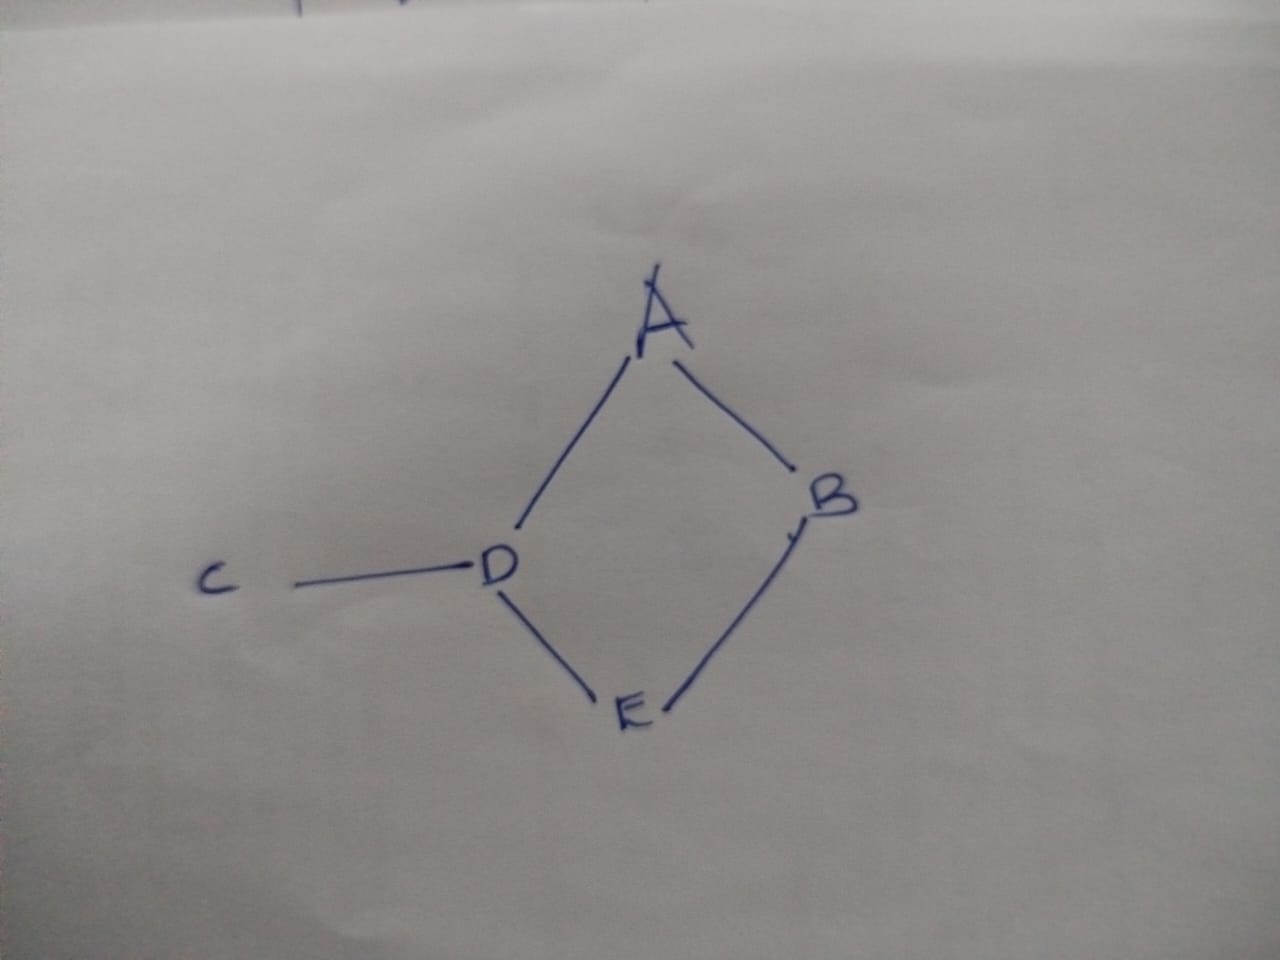
\includegraphics[width=0.8\textwidth]{graph.jpg}
    \]
    \end{enumerate}
    \item How many of the following statements are correct?
    \item \begin{enumerate}
        \item All cyclic graphs are complete graphs:\( \textbf{False} \) - A cyclic graph is a graph that contains a cycle. A complete graph is a graph in which each pair of distinct vertices is connected by a unique edge. A cyclic graph can be complete but not all cyclic graphs are complete.
        \item All complete graphs are cyclic graphs : \( \textbf{False} \) - A complete graph is a graph in which each pair of distinct vertices is connected by a unique edge. A cyclic graph is a graph that contains a cycle. A complete graph can be cyclic but not all complete graphs are cyclic.
        \item All paths are bipartite. \( \textbf{True} \) - A path is a trail with no repeated vertices and edges. A bipartite graph is a graph whose vertices can be divided into two disjoint sets such that no two vertices within the same set are adjacent. A path is a bipartite graph.
        \item There are cyclic graphs which are complete graphs. \( \textbf{True} \) - A cyclic graph is a graph that contains a cycle. A complete graph is a graph in which each pair of distinct vertices is connected by a unique edge. A cyclic graph can be complete.
    \end{enumerate}
    \item Which of the following statements for a simple graph is correct.
    \begin{enumerate}
        \item Every trail is a path (\(\textbf{False}\)) - A trail is a walk in which no edge is repeated but the vertices can be repeated. A path is a trail with no repeated vertices and edges. So every trail is a path.
        \item Every path is a trail (\(\textbf{True}\)) - A path is a trail with no repeated vertices and Edges but a trail \(\textbf{can}\) have repeated vertices and edges. So every path is a trail.
        \item path
        \item Path and trail have no relation
    \end{enumerate}
\end{enumerate}



\end{document}